\documentclass{article}
\usepackage{graphicx}
\usepackage{amsmath}
\usepackage{epsf}
\usepackage{color}
% titlepage causes separate title page
% our latex is biased off 1in vertically and horizontally
\newtheorem{theorem}{Theorem}
\setlength{\topmargin}{0.1in}
\setlength{\oddsidemargin}{0in}
\setlength{\evensidemargin}{0in}
\setlength{\headheight}{0in}
\setlength{\headsep}{0in}
\setlength{\textheight}{9in}
\setlength{\textwidth}{6.5in}
% require that floats fill 90% of a page in order for that page to be
% ``float-only''
\renewcommand{\dblfloatpagefraction}{0.9}
\renewcommand{\floatpagefraction}{0.9}
%\renewcommand{\baselinestretch}{1.2} % interline spacing
%\setlength{\parindent}{0in}
%\parskip=10pt plus2pt minus2pt
%\setlength{\unitlength}{0.1in}
%\pagestyle{empty} % no page numbering
\newenvironment{bibparagraph}{\begin{list}{}{ %
    \setlength{\labelsep}{-\leftmargin} %
    \setlength{\labelwidth}{0pt} %
    \setlength{\itemindent}{-\leftmargin} %
    \setlength{\listparindent}{0pt}}}{\end{list}}
\def\makefigure#1#2{\begin{figure}
\begin{center}
\input{#1}
\end{center}
\caption{#2}
\label{#1}
\end{figure}}

\def\limplies{\; \supset \;}
\def\land{\: \wedge \:}
\def\lor{\: \vee \:}
\def\iff{\; \equiv \;}
\def\lnot{\neg}
\def\lforall#1{\forall \: #1 \;}
\def\lexists#1{\exists \: #1 \;}
\def\glitch#1{{\tt #1}} % glitch on
%\def\glitch#1{} % glitch off
\def\comment#1{}
\def\pnil{[\;]}
\def\pif{\; \mbox{\tt :- } \;}
\def\tuple#1{$\langle #1\rangle$}
\def\mtuple#1{\langle #1\rangle}
\def\ceiling#1{\lceil #1\rceil}
\def\floor#1{\lfloor #1\rfloor}
\def\centerps#1{\begin{center}
\leavevmode
\epsfbox{#1}
\end{center}}
\def\argmax{\mathop{\rm argmax}}
\def\argmin{\mathop{\rm argmin}}
\def\grad{\nabla\!}
\def\celsius{^\circ\mbox{C}}
%\long\def\answer#1{}  % comment out for solutions
%\long\def\question#1{#1} % comment out for solutions
\long\def\answer#1{{\color {blue} {\sl #1}}}  % comment in for solution
\long\def\question#1{} % comment in for solution

\def\z{{\bf z}}
\def\x{{\bf x}}
\def\w{{\bf w}}

\begin{document}

\begin{titlepage}
    \begin{center}
        \vspace*{4cm}

        \textbf{\Large CS534 - Machine Learning}

        \vspace{0.5cm}
 
        \textbf{\Large Written Homework Assignment 2}
 
        \vspace{1cm}

        Author: Vy Bui

        OSUID: 934370552 \\ 
        
        Email: buivy@oregonstate.edu

        \vfill
             
        \vspace{0.8cm}
      
             
        The School of Electrical Engineering and Computer Science\\
        Oregon State University\\
             
    \end{center}
\end{titlepage}


%Please submit via TEACH electronically.
This assignment covers Perceptron, Kernel methods, SVMs and Naive Bayes
\begin{enumerate}
\item (Subgradient) (2 pts) Consider the $L_1$ form function for 
$\x\in R^d$: $f(\x)=|\x|_1=\sum_{i=1}^d|x_i|$. Show that 
${\bf g}=[g_1, g_2, ...,g_d]^T$ is a subgradient of $f(\x)$ at $\x={\bf 0}$ if 
every $g_i \in [-1,1] $ using the definition of subgradient: $g$ is a subgradient of $f(x)$ at $x_0$ if $\forall x$, $f(x)\geq f(x_0)+g^T(x-x_0)$

\answer{

}

\item (Perceptron) (2 pts) Consider the following argument. We know that the 
number of steps for the perceptron algorithm to converge for linearly separable 
data is bounded by $(\frac{D}{\gamma})^2$. If we multiple the input $\x$ by a 
small constant $\alpha$, which effectively reduces the bound on $|\x|$ to 
$D' =\alpha D$, we can reduce the upper bound to $(\alpha \frac{D}{\gamma})^2$. 
Is this argument correct? Why? 

\answer{Put your solution here.}

\item (Kernel or not). (9 pts) In the following problems, suppose that $K$, 
$K_1$ and $K_2$ are kernels with feature maps $\phi$, $\phi_1$ and $\phi_2$. 
For the following functions $K'(x, z)$, state if they are kernels or not. If 
they are kernels, write down the corresponding $\phi$ in terms of $\phi$, 
$\phi_1$ and $\phi_2$. If they are not kernels, prove that they are not.

\begin{itemize}
\item (2 pts) $K'(\x, \z) = cK(\x, \z)$ for $c > 0$.\\
\answer{Put your solution here.
}
\item (2 pts) $K'(\x,\z) = cK(\x, \z)$ for $c < 0$.\\
\answer{Put your solution here.}
\item (2 pts) $K'(\x,\z)= c_1K_1(\x, \z)+c_2K_2(\x,\z)$ for $c_1, c_2 >0$.\\
\answer{Put your solution here.}
\item (3 pts) $K'(\x,\z)= K_1(\x, \z)K_2(\x,\z)$ .\\
\answer{Put your solution here.
}

\end{itemize}
\item (Hard margin SVM) (5 pts) Apply linear SVM without soft margin to the 
following problem.
\begin{center}
\begin{figure}[h]
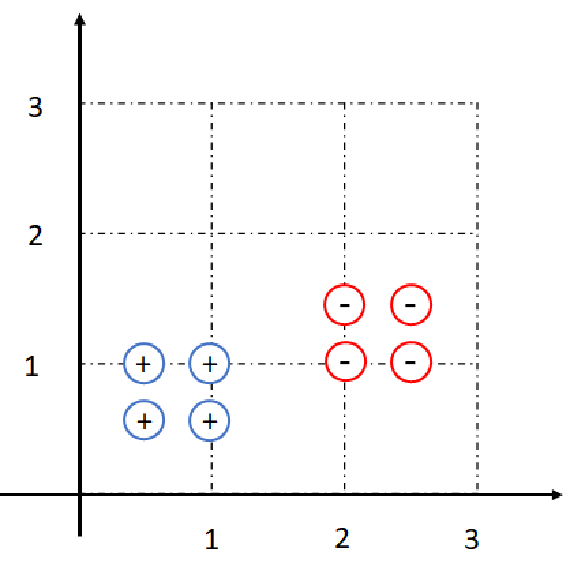
\includegraphics[width=3in]{svm.pdf}
\end{figure}
\end{center}

\begin{itemize} \item[a.] (2pts) Please mark out the support vectors, the 
decision boundary ($w_1x_1+w_2x_2 +b =0$) and $w_1x_1+w_2x_2+b =1$ and 
$w_1x_1+w_2x_2+b =-1$. You don't need to solve the optimization problem for 
this, you should be able to eyeball the solution and find the linear separator 
with the largest margin.

\answer{Put your solution here.
}
\item[b.] (3 pts) Please solve for $w_1, w_2$ and $b$ based on the support 
vectors you identified in (a). Hint: the support vectors would have functional 
margin = 1. \\
\answer{
Put your solution here.}
\end{itemize}
\item $L_2$ SVM (10 pts) \\
Given a set of training examples $\{(\x_i, y_i)\}_{i=1}^N$, where 
$y_i\in \{1, -1\}$ for all $i$. The following is the primal formulation of $L_2$ 
SVM, a variant of the standard SVM obtained by squaring the slacks.
\begin{align*}
\min_{\w, b, \xi} \mbox{ }& \frac{1}{2}\w^T\w+c\sum_{i=1}^N \xi_i^2 \\
\mbox{s.t. } & y_i(\w^T\x_i+b)\geq 1-\xi_i \mbox{,   } i \in \{1,\cdots,N\}\\
 & \xi_i\geq 0, \mbox{  }  i\in \{1,\cdots,N\}
\end{align*}

\begin{itemize}
\item [a.] (2pts) Show that removing the second constraint $\xi_i\geq 0$ will 
not change the solution to the problem. In other words, let 
$(\w^*, b^*, {\bf \xi}^*)$ be the optimal solution to the problem without this 
set of constraints, show that  
${\bf \xi}_i^* \geq 0$, $\forall i\in\{1,\cdots,N\} $. 
( Hint: use proof by contradiction by assuming that there exists 
some $\xi_i^*<0$.)\\

\answer{Put your solution here.}
\item [b.] (2 pts) After removing the second set of constraints, we have a 
simpler problem with only one set of constraints. Now provide the lagrangian of 
this new problem.\\
\answer{Put your solution here.}
\item [c.] (6pts) Derive the dual of this problem. How is it different from the 
standard SVM with hinge loss? Which formulation is more sensitive to outliers?\\
\answer{Put your solution here.
}

\end{itemize}
\item (Naive Bayes Classifier) (6 pts) Consider the following training set:
\begin{center}
\begin{tabular}{|c|c|c|c|}\hline
A&B&C&Y\\ \hline
0&1&1&0 \\ \hline
1&1&1&0 \\ \hline
0&0&0&0 \\ \hline
1&1&0&1 \\ \hline
0&1&0&1 \\ \hline
1&0&1&1 \\ \hline
\end{tabular}
\end{center}
\begin{enumerate}
\item (2 pts) Learn a Naive Bayes classifier by estimating
all necessary probabilities (there should be 7 independent probabilities to be 
estimated in total).

\answer{Put your solution here.
}
\item (3 pts) Compute the probability $P(y=1|A=1, B=0, C=0)$.
\answer{
Put your solution here.}
\item (1 pts) Suppose we know that the three features A, B and C are independent 
from one another, can we say that the Naive Bayes assumption is valid? (Note 
that the particular data set is irrelevant for this question). If your answer 
is yes, please explain why; if you answer is no please give an counter example.

\answer{Put your solution here.}

\end{enumerate}

\item (Naive Bayes learns linear decision boundary.) (6 pts) Consider a naive 
Bayes binary classifier with a set of binary features $x_1, x_2, ...,x_d$. Show 
that the Naive Bayes classifier learns a linear decision boundary 
$w_0+w_1x_1+w_2x_2+...+w_dx_d=0$. Express the weights using the Naive Bayes 
parameters. Hint: consider the decision rule of predicting 
$y=1$ if $P(y=1|\x) > P(y=0|\x)$. This is equivalent to having a decision 
boundary defined by $\log\frac{P(y=1|\x)}{P(y=0|\x)}=0$.

\answer{
Put your solution here.}
\end{enumerate}

\end{document}
